\begin{figure}[H]
  \begin{subfigure}[t]{\columnwidth}
  \centering
  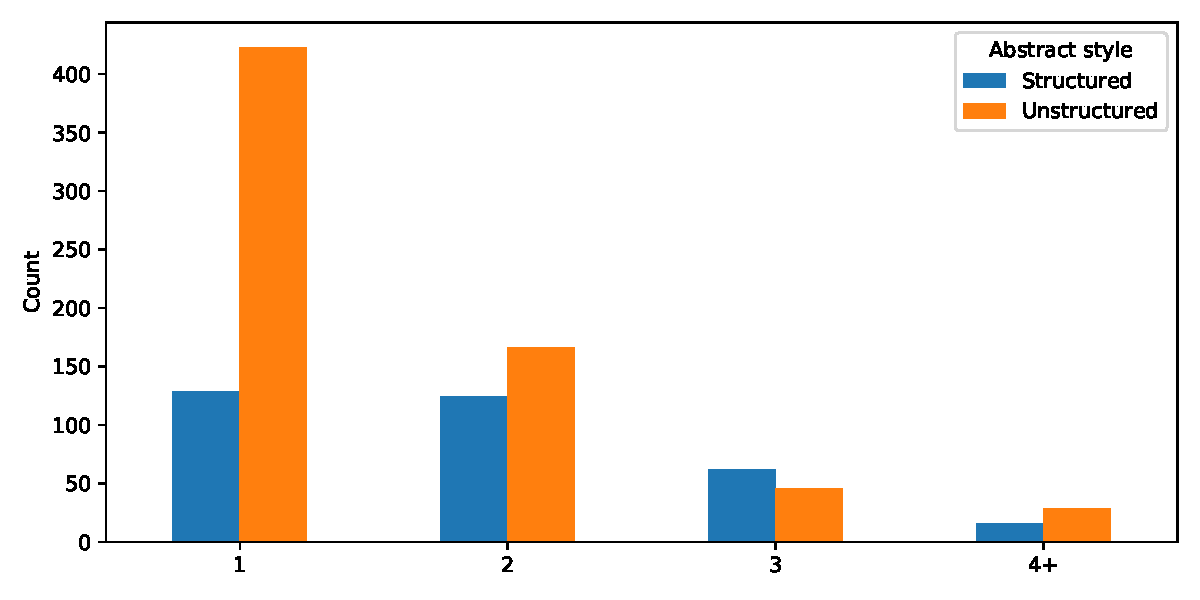
\includegraphics[width=\columnwidth]{figures/n-rationales.pdf}
  \caption{The number of rationales supporting each claim. For instance, roughly 150 unstructured abstracts contain 2 rationales.}
  \label{fig:n_rationales}
  \end{subfigure}

  % Largely redundant.
  % \begin{subfigure}[t]{\columnwidth}
  %   \centering
  %   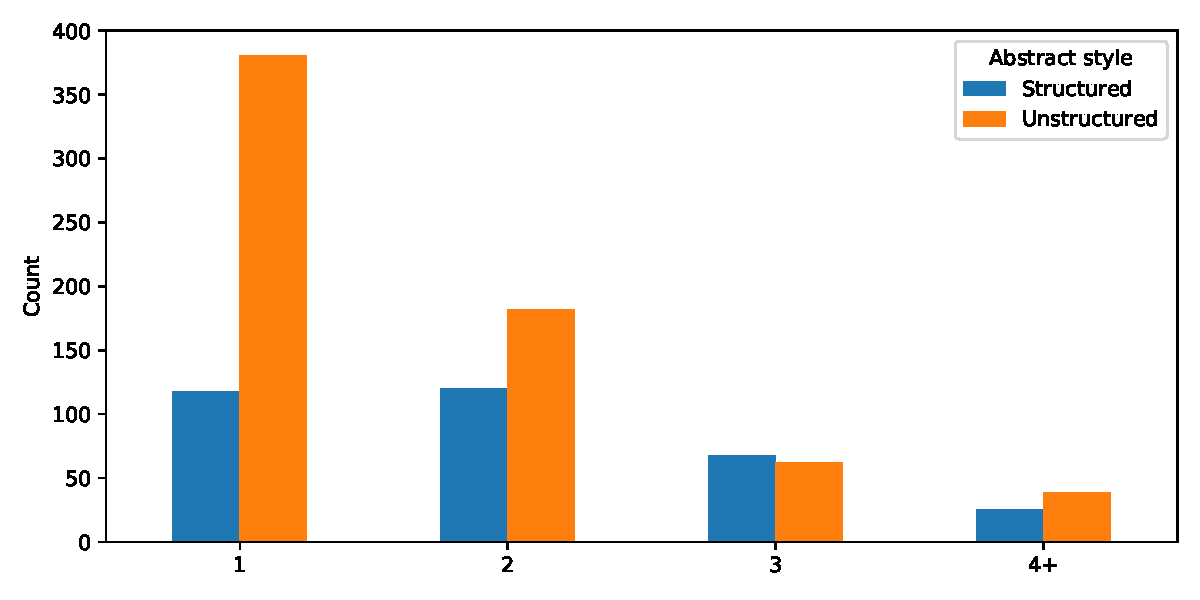
\includegraphics[width=\columnwidth]{figures/total-sentences.pdf}
  %   \caption{The total number of sentences supporting each claim.}
  % \end{subfigure}

  \begin{subfigure}[t]{\columnwidth}
    \centering
    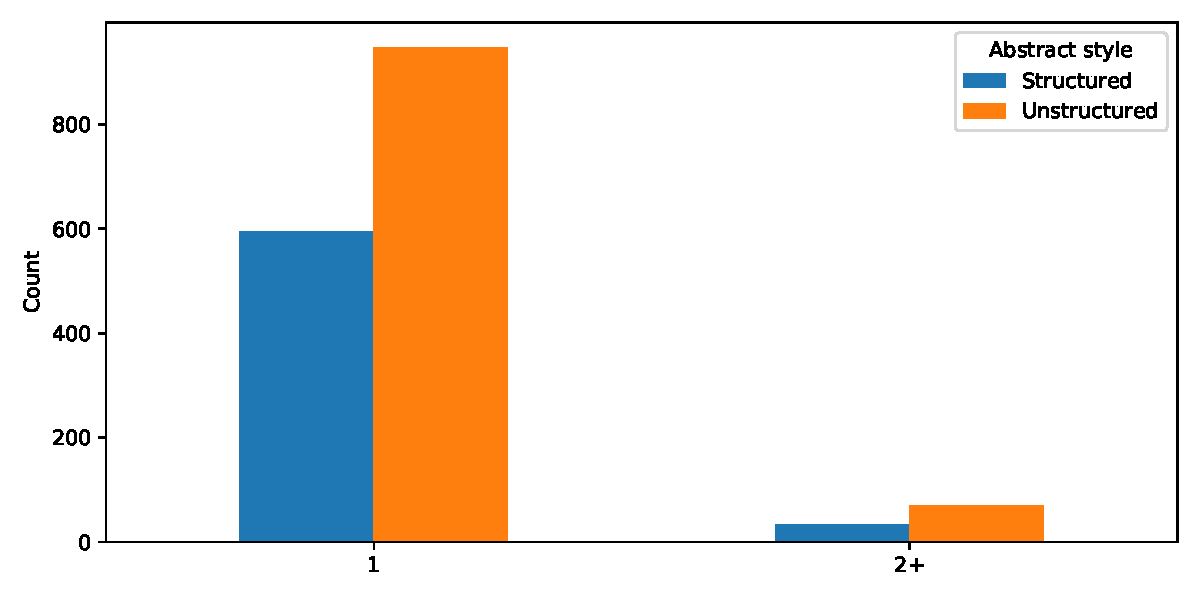
\includegraphics[width=\columnwidth]{figures/rationale-length.pdf}
    \caption{The number of sentences per rationale.}
    \label{fig:rationale_length}
  \end{subfigure}

  \label{fig:rationale_stats}
  \caption{Statistics on rationales. Most claims are supported by a single rationale, but structured abstracts are more likely to have two rationales. The great majority of rationales are a single sentence.}
\end{figure}